\documentclass[11pt,a4paper]{scrartcl}
\typearea{12}
\usepackage{graphicx}
\usepackage{pstricks}
\usepackage{listings}
\lstset{language=python}
\pagestyle{headings}
\newcommand{\turtle}{\texttt{Turtle}\,}
\newcommand{\lnn}[1]{\textbf{line #1}\,}
\newcommand{\Lnn}[1]{\textbf{Line #1}\,}
\markright{Python turtle worksheet}
\begin{document}
\subsection*{Introduction}
Here is a simple turtle programme (\texttt{turtle\_doing\_nothing.py}):
\begin{lstlisting}[numbers=left]
from turtle import *

tom=Turtle()

tom.getscreen()._root.mainloop()
\end{lstlisting}
\Lnn{1} and \lnn{5} aren't worth spending much time on at first, the first
line imports the library of commands related to turtle, \lnn{5}
prevents the computer from closing the graphics window when the
programme has finished running; we won't include this line again,
though it is needed. \Lnn{3} is important, it tells the computer to
make an object, in this case a \turtle and call it \texttt{tom}, it
knows what a \turtle is from the library it imported in line 1; in the
instructions on what to do when making a \turtle the computer is told
to open a graphics window and to draw the turtle, a little arrow
shape.
\begin{center}
\fbox{

\includegraphics[width=10cm]{code/turtle_doing_nothing.eps}}
\end{center}

Here the turtle does something (\texttt{line.py}):
\begin{lstlisting}[numbers=left]
from turtle import *

tom=Turtle()

tom.forward(100)
\end{lstlisting}
The extra line, \lnn{5}, tells the turtle to move forward by 100 units,
this is an important piece of Python syntax, to tell an object to do
something you use a dot followed by the command, here it tells the
\turtle called \texttt{tom} to perform the command
\texttt{forward}. Of course, the command has to make sense for
whatever type of object it is dotted onto, but here it does,
\texttt{forward} is one of the defined commands for a \turtle object.
\begin{center}
\fbox{
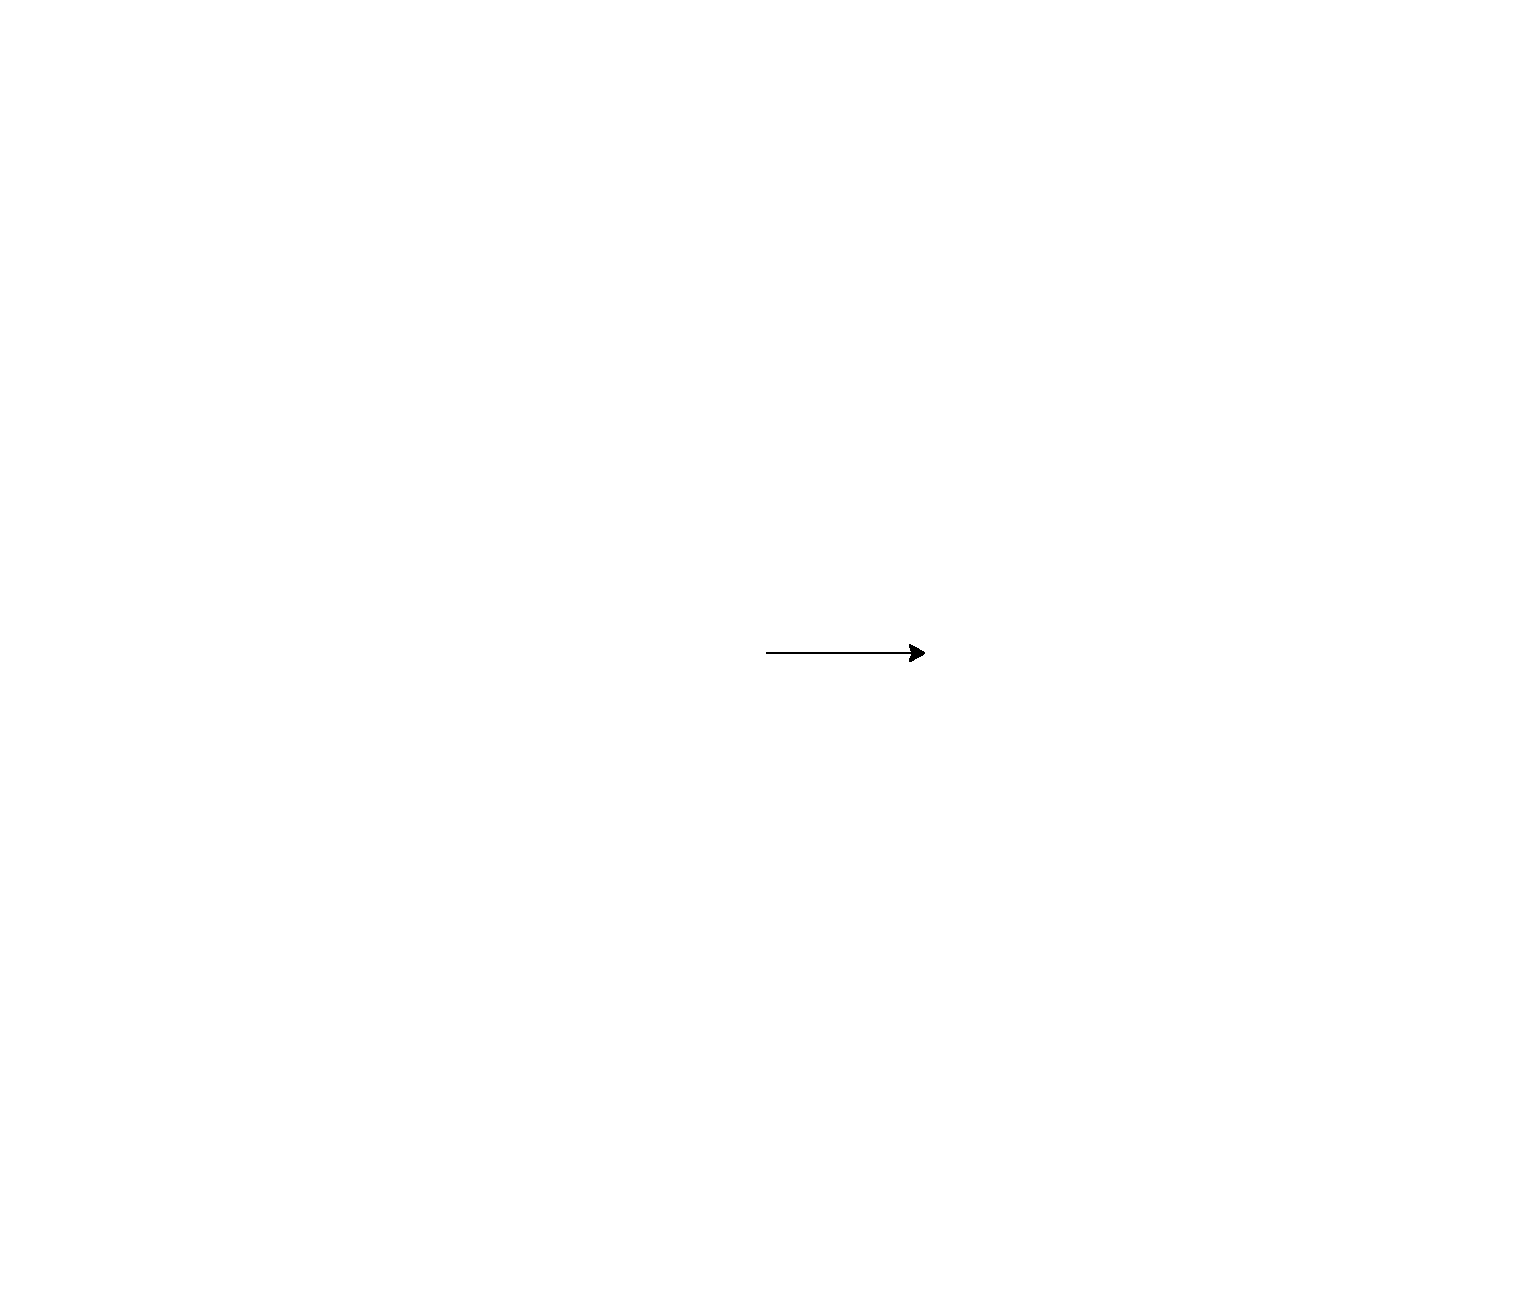
\includegraphics[width=10cm]{code/line.eps}}
\end{center}

\turtle objects have another command \texttt{right(90)} which turns the turtle by $90^\circ$. QUESTION: Can you write a programme to draw this:
\begin{center}
\fbox{
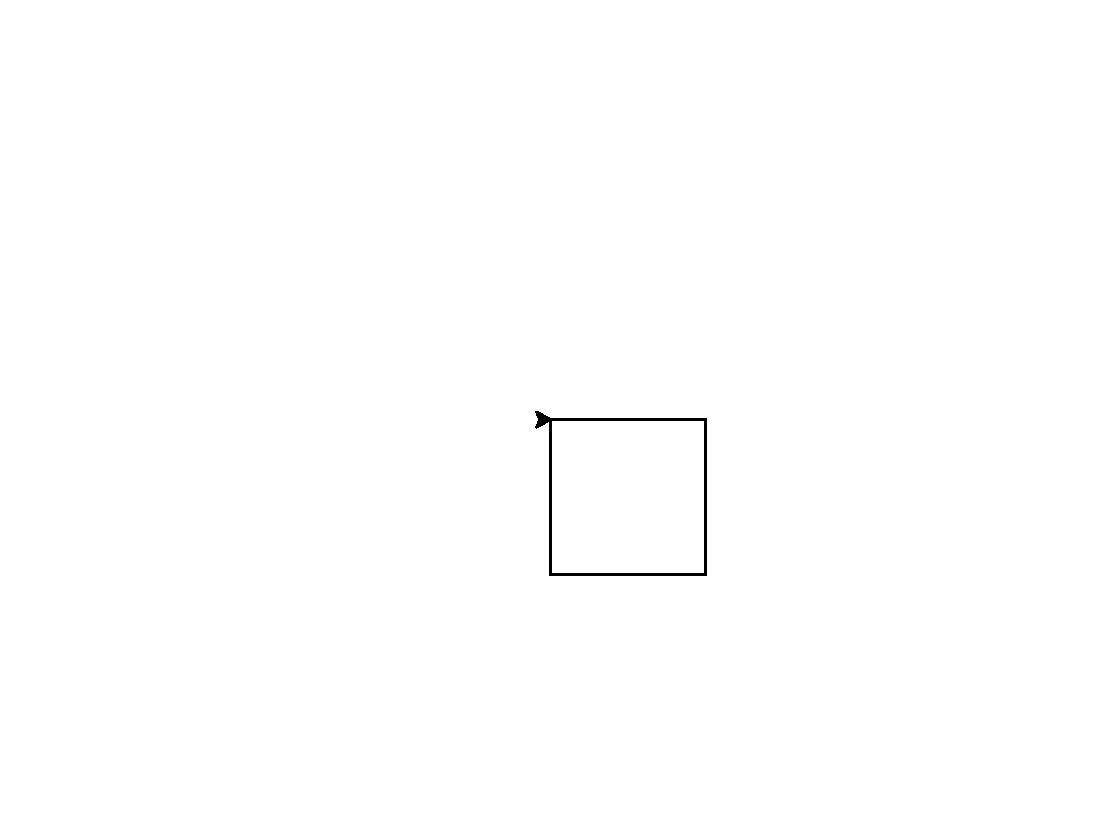
\includegraphics[width=10cm]{code/right_angle.eps}}
\end{center}
QUESTION: How about a square?
\begin{center}
\fbox{
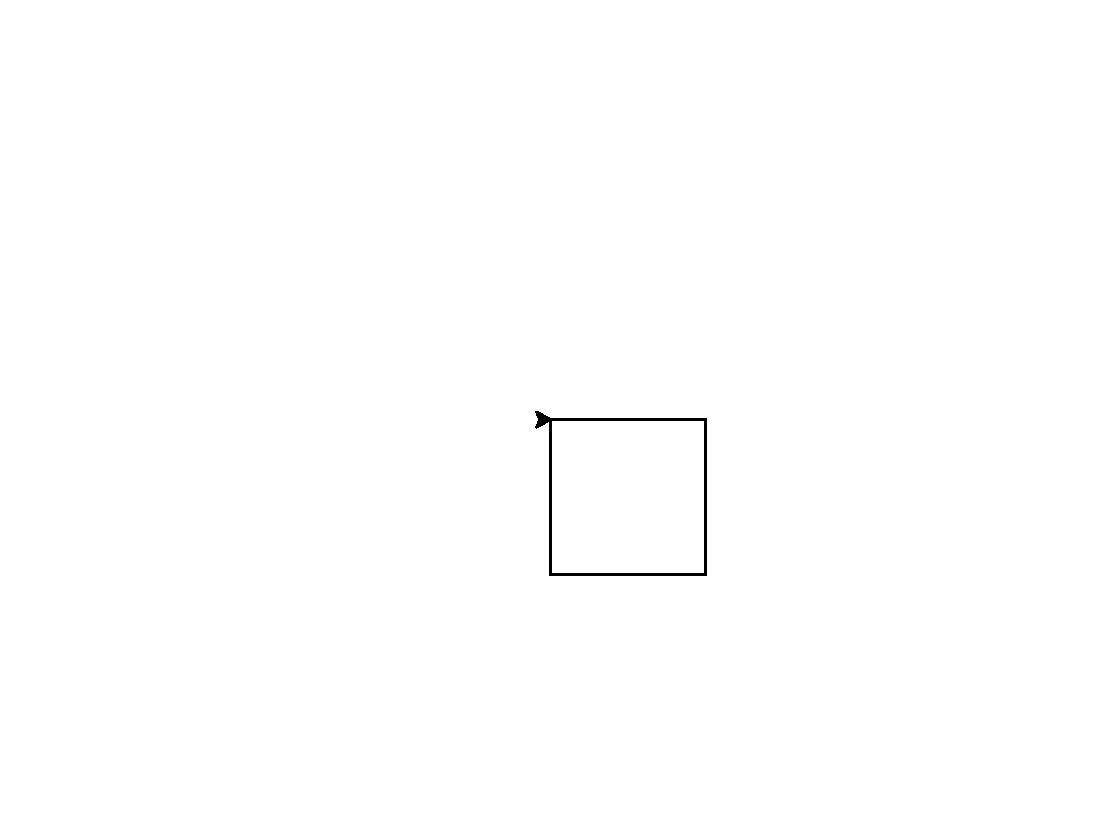
\includegraphics[width=10cm]{code/square.eps}}
\end{center}

Perhaps you programme to draw a square looked like this
\begin{lstlisting}[numbers=left]
from turtle import *

tom=Turtle()

tom.forward(100)
tom.right(90)
tom.forward(100)
tom.right(90)
tom.forward(100)
tom.right(90)
tom.forward(100)
tom.right(90)
\end{lstlisting}
There are two problems with this, most obviously it is boring writing
in the same two lines again and again; secondly, the programme is
inflexible and hard to read, we'll deal with the inflexible bit later,
but as for the hard to read, to know that it draws four lines and has
four corners you need to count the lines; it would be better if the
\lq{}fourness\rq{} was more apparent, as it is in this programme (\texttt{square\_loop}):
\begin{lstlisting}[numbers=left]
from turtle import *

tom=Turtle()

for i in range(0,4):
   tom.forward(100)
   tom.right(90)

\end{lstlisting}
The business part of this program is \textbf{line 5};
\texttt{range(0,4)} is the list of numbers \texttt{[0,1,2,3]}, so
starting at zero and ending one before four; the full command says
that \texttt{i} takes each value in this list in turn and then does
all the stuff belonging to the command. Here the command is a
\texttt{for}, a command that says \lq{}do everything that belongs to
the for once for every value the variable, in this case i, is
instructed to take\rq{}. In Python stuff belonging to a command is
indented, so that means it does \lnn{6} and \lnn{7} once for each item
in the list, that is four times. Of course, in this programme
\texttt{i} isn't used for anything except counting but it could be
(\texttt{spiral1.py}):
\begin{lstlisting}[numbers=left]
from turtle import *

tom=Turtle()

for i in range(0,8):
   tom.forward(100+10*i)
   tom.right(90)

\end{lstlisting}
giving
\begin{center}
\fbox{
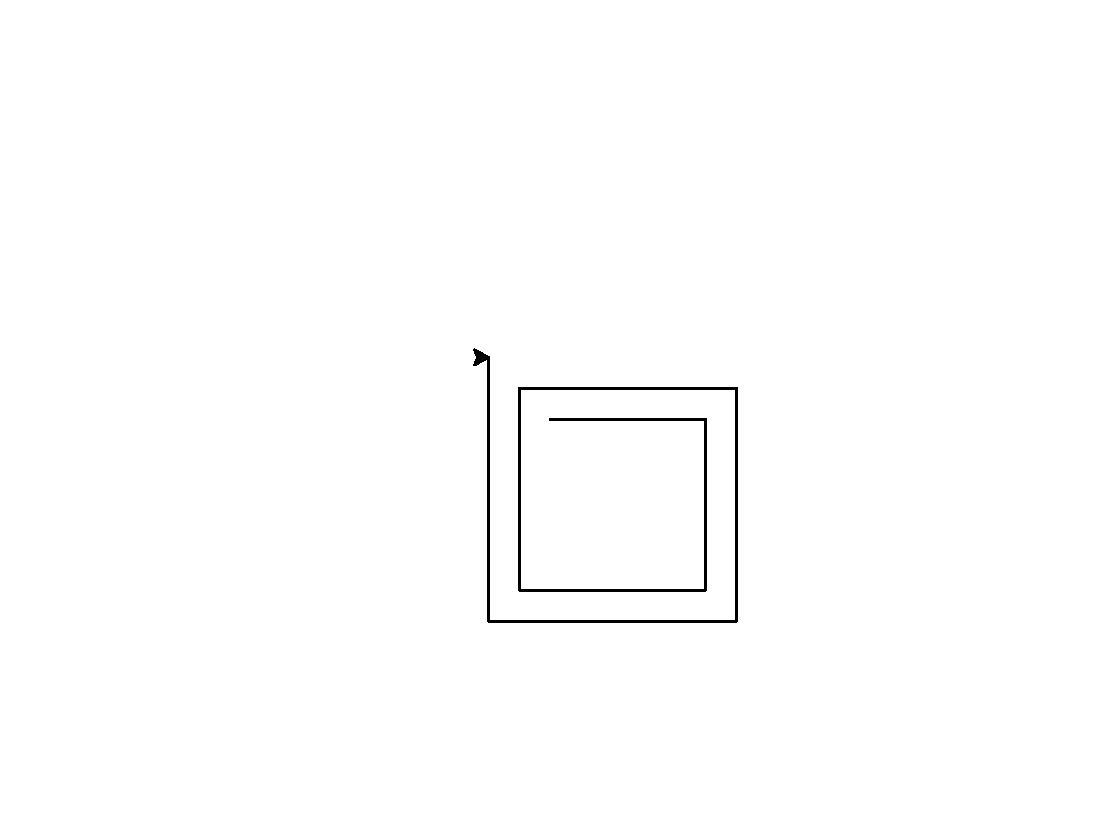
\includegraphics[width=10cm]{code/spiral1.eps}}
\end{center}
\texttt{i} is variable, it stores some data, in this case a number
which changes each time the programme goes around the \texttt{for}
loop. Once slightly confusing thing is \lq{}scoping\rq{}, which is
where the variable is defined; the \texttt{i} is only defined inside
the \texttt{for} loop, that is, it only exists while the programme is
executing \lnn{5} to \lnn{7}, but that's fine, that's where we use it.
QUESTION: Can you draw a triangular spiral like this:
\begin{center}
\fbox{

\includegraphics[width=10cm]{code/spiral2.eps}}
\end{center}


\end{document}

